\documentclass[10pt]{article} 
\usepackage[T1]{fontenc}
\usepackage{amsmath}
\usepackage{graphicx}
\usepackage[font=small,skip=3pt]{caption}
\usepackage{amsxtra}
\usepackage{empheq}
\usepackage{amsfonts}
\usepackage{amssymb}
\usepackage{amsthm}
\usepackage{enumitem}
%\usepackage{tcolorbox}
\usepackage{url}
\usepackage{color,hyperref}
%\usepackage{pgf, tikz}
\usepackage{tikz-cd}
\usepackage{epstopdf}
%\usepackage{pgfplots}
%\usepackage{mathrsfs}
\usetikzlibrary{calc,arrows,decorations.pathmorphing}
\hypersetup{colorlinks,breaklinks,
             linkcolor=blue,urlcolor=blue,
           anchorcolor=blue,citecolor=blue}

\usepackage[margin=3cm]{geometry}
\newcommand{\eps}{\varepsilon}
\newcommand{\Z}{\mathbb{Z}}
\renewcommand{\L}{\mathcal{L}}
\newcommand{\N}{\mathbb{N}}
\newcommand{\R}{\mathbb{R}}
\newcommand{\C}{\mathbb{C}}
\newcommand{\Q}{\mathbb{Q}}
\newcommand{\E}{\mathbb{E}}
\newcommand{\prob}{\mathbb{P}}
\newcommand{\limn}{\lim_{n\to \infty}}
\newcommand{\limsupn}{\limsup_{n \to \infty}}
\newcommand{\liminfn}{\liminf_{n \to \infty}}
\newenvironment{bp}{\color{blue}\begin{proof}}{\end{proof}}
\newenvironment{bs}{\color{blue}\begin{proof}[Solution]}{\end{proof}}
\renewcommand{\bar}[1]{\overline{#1}}
\renewcommand{\Im}{\text{Im}}
\renewcommand{\Re}{\text{Re}}
\newcommand{\vb}[1]{\mathbf{#1}}
\newcommand{\dudn}{\frac{\partial u}{\partial n}}
\newtheorem{theorem}{Theorem}[section]
\newtheorem{lemma}[theorem]{Lemma}
\newcommand{\limh}{\lim_{h\to 0^{+}}}
\newcommand{\lp}{\left(}
\newcommand{\rp}{\right)}
\newcommand{\lb}{\left[}
\newcommand{\rb}{\right]}
\newcommand{\open}{\mathcal{O}}
\newcommand{\hotempty}{\varnothing}
\newcommand{\tpose}{\mathsf{T}}
\DeclareMathOperator*{\argmin}{arg\,min}
\DeclareMathOperator*{\argmax}{arg\,max}
 

\def\scriptf{{\mathcal F}}
\def\scriptq{{\mathcal Q}}
\def\scriptg{{\mathcal G}}
\def\scriptm{{\mathcal M}}
\def\scriptb{{\mathcal B}}
\def\scriptc{{\mathcal C}}
\def\scriptt{{\mathcal T}}
\def\scripti{{\mathcal I}}
\def\scripte{{\mathcal E}}
\def\scriptv{{\mathcal V}}
\def\scriptw{{\mathcal W}}
\def\scriptu{{\mathcal U}}
\def\scriptS{{\mathcal S}}
\def\scripta{{\mathcal A}}
\def\scriptr{{\mathcal R}}
\def\scripto{{\mathcal O}}
\def\scripth{{\mathcal H}}
\def\scriptd{{\mathcal D}}
\def\scriptl{{\mathcal L}}
\def\scriptn{{\mathcal N}}
\def\scriptp{{\mathcal P}}
\def\scriptk{{\mathcal K}}
\def\scriptP{{\mathcal P}}
\def\scriptj{{\mathcal J}}
\def\scriptz{{\mathcal Z}}
\def\scripts{{\mathcal S}}
\def\scriptx{{\mathcal X}}
\def\scripty{{\mathcal Y}}
\def\frakv{{\mathfrak V}}
\def\frakG{{\mathfrak G}}
\def\frakB{{\mathfrak B}}
\def\frakC{{\mathfrak C}}

\def\symdif{\,\Delta\,}
\def\mustar{\mu^*}
\def\muplus{\mu^+}

%%% AVERAGE INTEGRAL %%%
\def\Xint#1{\mathchoice
{\XXint\displaystyle\textstyle{#1}}%
{\XXint\textstyle\scriptstyle{#1}}%
{\XXint\scriptstyle\scriptscriptstyle{#1}}%
{\XXint\scriptscriptstyle\scriptscriptstyle{#1}}%
\!\int}
\def\XXint#1#2#3{{\setbox0=\hbox{$#1{#2#3}{\int}$ }
\vcenter{\hbox{$#2#3$ }}\kern-.6\wd0}}
\def\ddashint{\Xint=}
\def\dashint{\Xint-}


\newcommand{\loc}{L^{1}_{\text{loc}}}
\newcommand{\acc}{\text{acc}}
\newcommand{\Var}{\operatorname{Var}}
\newcommand{\Ker}{\operatorname{Ker}}
\newcommand{\rank}{\operatorname{rank}}
\newcommand{\Arg}{\operatorname{Arg}}
\newcommand{\Res}{\operatorname{Res}}
\newcommand{\abserr}{\operatorname{abserr}}
\newcommand{\relerr}{\operatorname{relerr}}
\newcommand{\round}{\operatorname{round}}
\newcommand{\sinc}{\operatorname{sinc}}
\newcommand{\sgn}{\operatorname{sgn}}
\newcommand{\wt}{\widetilde}
\newcommand{\wh}{\widehat}



\newtheorem*{thm*}{Theorem}
\definecolor{ccqqqq}{rgb}{0.8,0.,0.}
\definecolor{uuuuuu}{rgb}{0.26666666666666666,0.26666666666666666,0.26666666666666666}
\definecolor{zzttqq}{rgb}{0.6,0.2,0.}
\definecolor{qqqqff}{rgb}{0.,0.,1.}
%\pgfplotsset{width=10cm, compat=1.9}

\begin{document}

{ \large \textbf{\textsc{High Performance Computing -- Problem Set 5 (Due May 4)}}}

{ \large \textbf{\textsc{solutions by Frederick Law}}}

\thispagestyle{empty}
\vspace{0.1in}


\begin{enumerate}

\item \textbf{MPI-parallel two-dimensional Jacobi smoother.} We implement a distributed memory parallel version of the two-dimensional Jacobi smoother from the second assignment. This is an extension of the one-dimensional case available in the class repository. We will use a uniform domain splitting and exchange unknowns corresponding to neighboring points (ghost points) on different processors. To make our lives easier, we only consider uniform splittings of all unknowns using $p = 4^{j}$, $j=0, 1, \dotsc, $ processors. Additionally, we assume that we deal with $N = 2^{j} N_{l}$ unknowns in the $x$ and $y$ directions, such that each processor works on $N_{l}^{2}$ unknowns. Before you start coding, figure out a few things:
\begin{itemize}
	\item For any $p$, find which points (and thus unknowns) must be update by which MPI tasks.
	\item Find which points much be communicated (i.e., the ghost nodes), and between which processors this communication must take place.
	\item I suggest following our one dimensional example with blocking sends and receives by allocating $(N_{l} + 2)^{2}$ unknowns for each MPI task. The "inner" $N_{l}^{2}$ points are processed by each MPI tasks, while the outer points are used to store and update the ghost point copies from neighboring MPI tasks.
\end{itemize}

Run your implementation on Prince. For large $N_{l}$ (e.g. $N_{l} = 100$), perform a weak scaling study and plot the timings (fix the number of iterations for this study) as you increase the number of points and MPI tasks. Then choose $N_{l}$ as large as possible to fit on one processor, and perform a strong scaling study, i.e., keep the problem size unchanged while increasing the number of MPI tasks, and plot the speedup compared to the ideal speedup.

\textbf{Solution:} We saved our implementation in \texttt{jacobi2D-mpi.cpp}. The implementation is straightforward, essentially following the Jacobi 2D implementation we did for a previous homework. The difference here is that now each MPI task has its own local grid, of size $(N_{l}+2)^{2}$. At the end of each iteration, we run 4 if loops to have all processes send the appropriate ghost points left, right, up, and down. These are done with the standard blocked sends and receives. 



% If you have difficulties compiling with .eps graphics, comment them out and use the also included .pdf versions.
\begin{figure}[!ht]
\begin{center}
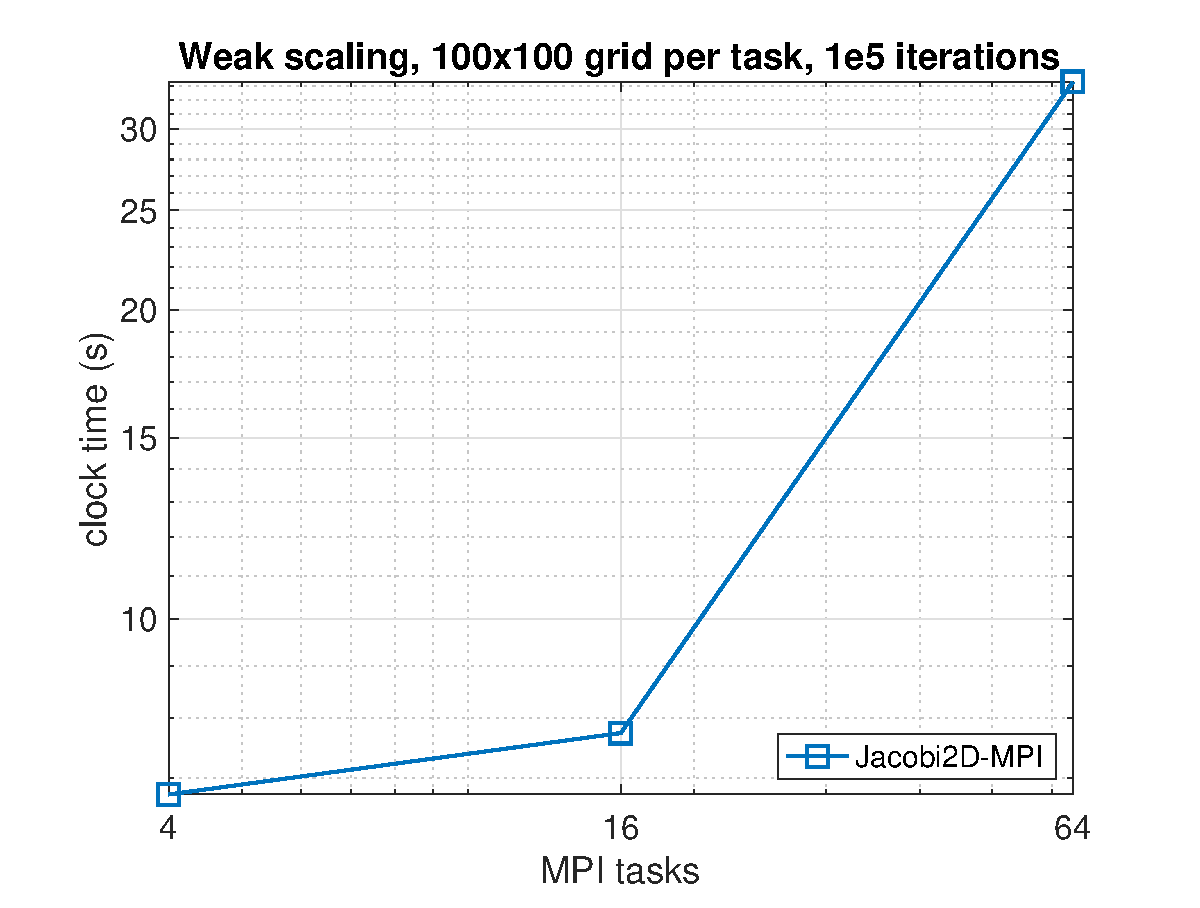
\includegraphics[scale=0.39]{weakscaling_small.eps}
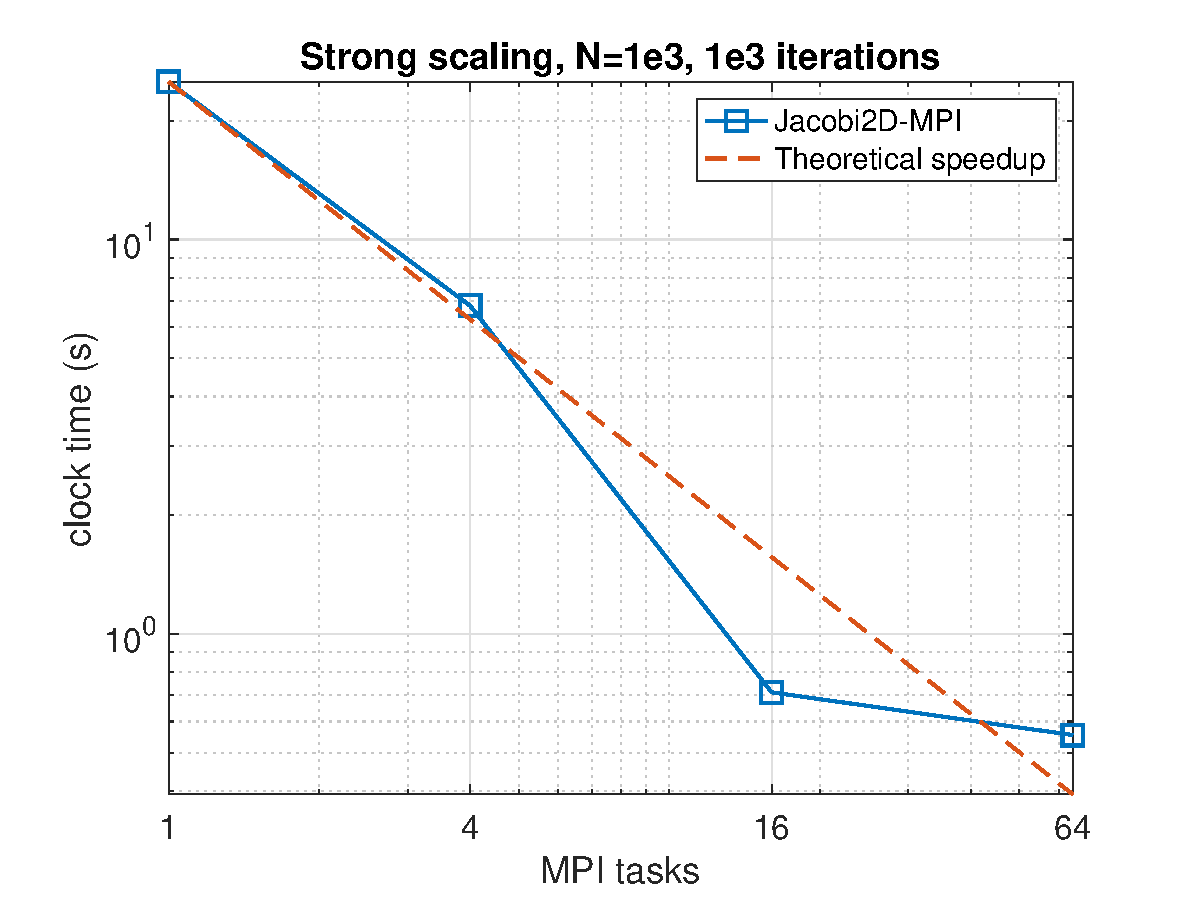
\includegraphics[scale=0.39]{strongscaling_small2.eps}
%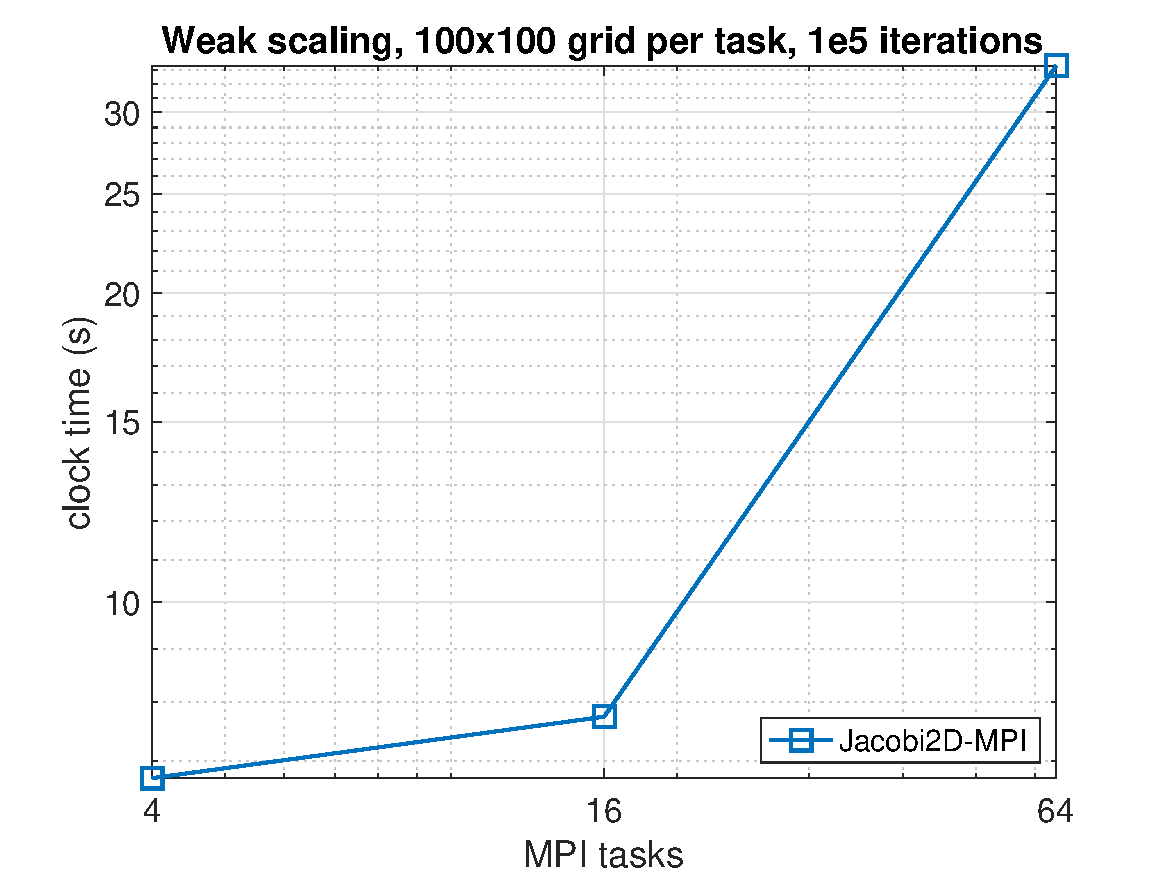
\includegraphics[scale=0.39]{weakscaling_small-eps-converted-to.pdf}
%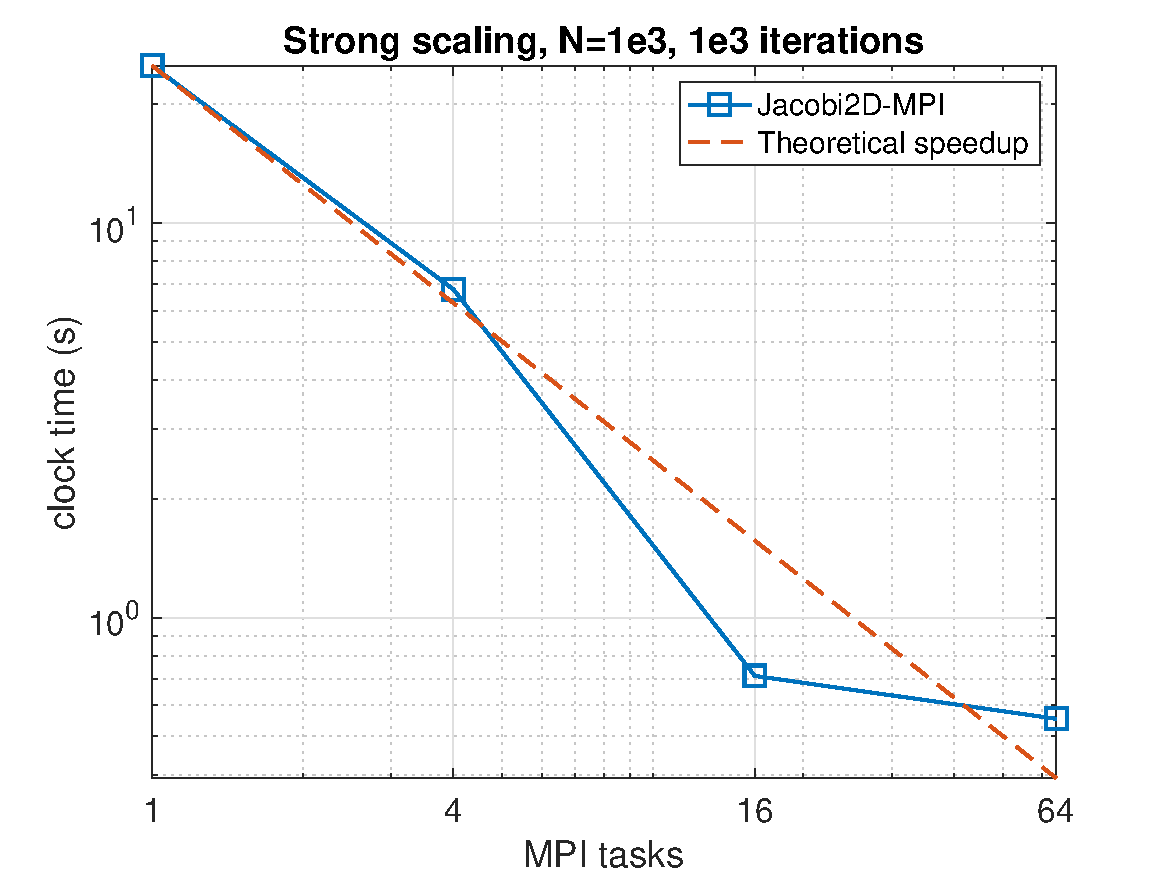
\includegraphics[scale=0.39]{strongscaling_small2-eps-converted-to.pdf}
\end{center}
\caption{\textbf{Left:} Weak scaling, with $N_{l} = 100$ for every MPI task. \textbf{Right:} Strong scaling, with $N = 1000$ fixed even as the number of tasks grows. All timings obtained on \texttt{c01\_17} partition of NYU Prince. In weak scaling we see that there is a jump in the runtime as we go from 16 to 64 MPI tasks. This corresponds to going from 1 node with 16 tasks, to 4 nodes with 16 tasks each (due to size restrictions on the nodes).}
\label{scaling-studies}
\end{figure}

We note that we store our local arrays in row-major order, so we need a secondary buffer to preload in the left / right ghost nodes to send. When sending or receiving from above or below however, we can just pass in the memory address of that piece of the local array. Computing the residual is done with an \texttt{MPI\_Allreduce}.

In Figure \ref{scaling-studies} we show the results of both a weak and strong scaling study, with all timings performed on the \texttt{c01\_17} partition of NYU Prince. In the weak scaling study, we use $N_{l} = 100$ fixed, and test using 4, 16, and 64 MPI tasks for 1e5 iterations. In this case, the number of total points increases, but each process works with a $100 \times 100$ grid. We see that the timings are similar for 4 and 16 MPI tasks, but there is a spike in clock time when we move to 64 tasks. One reason for this is that when doing 64 tasks, we must now use 4 nodes with 16 tasks each, and the inter-node communication may have extra overhead.

In our strong scaling study, we fix $N = 1000$ for 1e3 iterations. Here we see that using 16 tasks we are able to get speedup faster than the theoretical, but 64 tasks yields speedup slow than theoretical. Again, one reason for this may be that the inter-node communication at 64 MPI tasks causes excessive overhead. Despite the results of the weak scaling study which show a spike in times for 64 MPI tasks, we see that our code scales fairly well in performance up to 64 nodes.






\item \textbf{Parallel sample sort.} Each of the $P$ processors creates an $N$-vector of ranom numbers. The target is to sort the union of all these distributed vectors; this union, let's call it $\vb v$, consists of $PN$ numbers and is assumed to be too large to fit into the memory of a single processor -- thus, a serial sort algorithm cannot be used. The goal is to sort $\vb v$ such that every processor roughly holds about $N$ sorted number, say $\vb v_{i}$, and that all elements on the processor with rank $i$ are smaller than those on the processor with rank $i+1$ (for all $i=0,1,\dotsc, P-2$). The above repository contains a stub called \texttt{ssort.cpp}. This file also contains an outline of the algorithm, which we also discussed in class. For a summary of the sample sort algorithm, see the Wikipedia entry for sample sort, as well as the pages linked under "References" from there. The main steps of sample sort are:
\begin{itemize}
	\item \textit{Select local samples:}  Each of the $P$ processors sorts the local array and selects a set of $S$ entries uniformly and communicates these entries to the root processor, who sorts the resulting $SP$ entries and determines $P-1$ splitters $\{ S_{1}, \dotsc, S_{P-1} \}$, which it broadcasts to all other processors.
	
	\item \textit{Distribute to buckets:} Each processor determines the "buckets" to which each of its $N$ elements belong; for instance, the first bucket contains all the numbers $\leq S_{1}$, the second one are all the entries that are in $(S_{1}, S_{2}]$ and so on. The numbers contained in each bucket are then communicated; processor 0 receives every processor's first bucket, processor 1 gets every processor's second bucket, and so on.
	
	\item \textit{Local sort:} Each processor uses a local sort and writes the result to disc.
	
\end{itemize}

Include the MPI rank in the file name. Run your implementation of the sorting algorithm on at least 64 cores of Prince, and present timings depending on the number of elements $N$ to be sorted per processor (report results for $N=10^{4}, 10^{5},\text{ and } 10^{6}$).

\textbf{Solution:} Our implementation followed the structure of the stud in \texttt{ssort.cpp}. We do a local sort, find uniform splitters, and then use an \texttt{MPI\_Gather} to put all the local splitters on the root process. The root process sorts these splitters, and uniformly picks $P-1$ global splitters from them. We use an \texttt{MPI\_Bcast} to send these global splitters to all nodes. 

We use \texttt{std::lower\_bound} to determine the number of data each task sends to every other task. Then we use first an \texttt{MPI\_Alltoall} to communicate the number of data each task expects to send and receive, allocate the appropriate space to receive, and then use an \texttt{MPI\_Alltoallv} to communicate the data. We then do a final sort, and write to disc as "output[rank].txt". 

We timed our method using 64 MPI processes on the \texttt{c01\_17} partition of NYU Prince for $N=1$e4, 1e5, 1e6 (not including the time needed to write to disc). Results are shown in Table \ref{ssort}.
\begin{table}[!ht]
\begin{center}
\caption{Timings of parallel sample sort using 64 MPI tasks on \texttt{c01\_17} partition of NYU Prince.}
\begin{tabular}{ |c | c | c |}
\hline
 $N=1$e4 & $N=1$e5 & $N=1$e6\\
\hline
0.057034 s& 0.074858 s& 0.620412 s\\
\hline
\end{tabular}
\label{ssort}
\end{center}
\end{table}

Looking at the results in Table \ref{ssort} we see that going from $N=1$e4 to $N=1$e5, we don't see much change, the timings are of the same order of magnitude. However, in moving from $N=1$e5 to $N=1$e6, we do see that the the timing increases. That is, the timing to sort $N=1$e6 is around 10 times longer than $N=1$e5 which is to be expected. Hence, this is an indication that inter-node communication does indeed incur a fair amount of overhead, so much so that we only see scaling for large $N$. For smaller values of $N$, such as $N=1$e4, we expect the run time to be dominated by this communication overhead.


\end{enumerate}
	
%\begin{thebibliography}{9}

%\bibitem{fem}
%S. Boyd and L. Vandenberghe.
%\textit{Convex Optimization}.
%Cambridge University Press 2004.

%\bibitem{john}
%S. G. Johnson.
%\textit{Notes on FFT-based differentiation}.
%2011.

%\end{thebibliography}




    
    


\end{document}

